\section{Templates}




\subsection{Boat}
The boat template is a model of a real boat. 
The boat is capable of carrying at most two persons and most have at least one adult to handle the boat. 
From the initial state, named Still, the only possible edge is to the OnePerson location. 
In this edge the boat calls for a handshake on the adultOn channel. 
Only persons responds to this and only one person can respond to a handshake.
A transition is made when a person responds to the handshake.  
When a person responds to the handskake the persons sailing time is transmitted through the global variable temp\_sailtime. 
This is necessary since UPPAAL does not support value parsing through channels. 
A function set\_sailtime is used to set the sailtime to the lowest value, so the sailing time of the fastest person is the one used. 
The function set\_sailtime compares the received sail time to the one already set on the boat. 
temp\_sailtime is reset to reduce the state space.
From the OnePerson location there are three edges. 
Two edges to the TwoPerson location where either a child or an adult embarks. 
The adultOn edge is similar to the first edge described. 
The childOn edge does not need to synchronize a sail time since the children cannot handle the boat. 
From both the TwoPerson and the OnePerson location an edge to the Sailing location is possible. 
Here a guard calls the function verify, which is described in figure\ref{fig:boat}. 
The Sailing location has an invariant that makes sure it stays in the location for at least the time it takes for the person to sail across. 
The only possible edge from the Sailing location is to the Arrived location. 
This edge has a guard to make sure that the boat arrives when it has stayed in the Sailing location in a period equivalent to the sail\_time. 
The edge broadcasts on allDisembark, which makes all persons on the boat disembark. 
The local variable boatL changes boolean value to note that the boat has changed site. 
After the disembarkment the sail\_time is reset to the maximum sail time and the position of the persons is verified using the verify function. 
\begin{figure}%
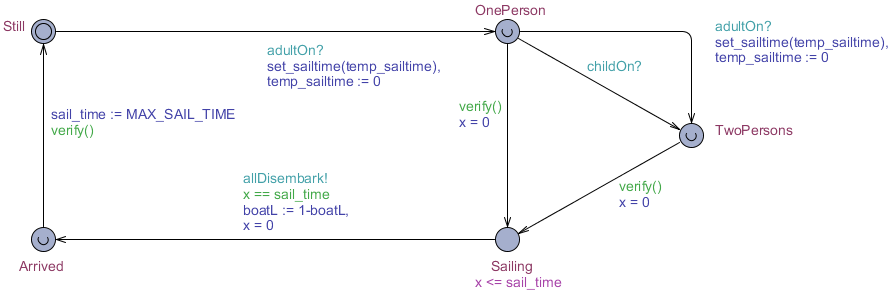
\includegraphics[width=\columnwidth]{pictures/boat.png}%
\caption{The boat template}%
\label{fig:boat}%
\end{figure}
















\subsection{Person}
The person model encapsulate a single person.
When instantiated it takes three arguments.
These arguments determines which type of person is being instantiated and how it should interact with the rest of the system.
The arguments that a person needs to be instantiated are: A channel, a person type, and a sail time.
The channel argument is used to signal that the given instance gets on the boat.
The person type indicates what kind of person is being instantiated, e.g. a boy.
The sail time is only applicable to the mom, dad, and police officer.
It is part of the 2nd task, which is to add temporal constraints and have each of the adults cross the river with different speeds.
\begin{figure}%
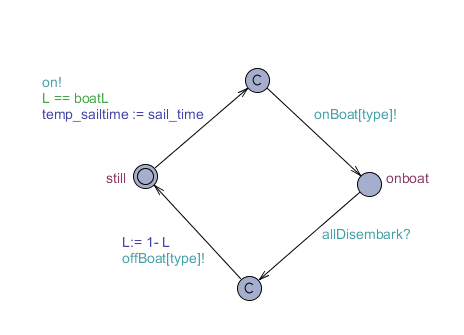
\includegraphics[width=\columnwidth]{pictures/person.png}%
\caption{The timed automata for a person}%
\label{fig:person}%
\end{figure}

The timed automata of a person seen in Figure \ref{fig:person} shows four circular connected locations.
The two locations OnBoat and OnLand indicate the current position of the person.
These names should be self-explanatory.
The local variable L is used to indicate which side of the river the person is on.
0 is left and 1 is right.
This variable is used to check that a person instance can only embark when it is on the same side as the boat.
L is update when a person as crossed the river and enters the location OnLand again.

The locations ToBoat and ToLand are intermediate states.
These are needed because there is a handshake with the boat and a broadcast to the observer whenever a person embarks or disembarks.
When a person embarks the reader can think of it as the person first jumps on the boat (taking the edge from OnLand to ToBoat) and immediately afterward reports to the observer (taking the edge from ToBoat to OnBoat).
Similarly when a person instance disembark it starts out by leaving the boat (or rather being forced to leave, since it is the boat that does the output on the allDisembark channel) and then reports to the observer.
















\subsection{Observer}
The purpose of the observer is to keep track of where the different persons are located. It maintains the following three arrays:
\begin{itemize}
	\item[\textbf{left}] Is an array with a list of all the person on the original shore
	\item[\textbf{right}] Contains a list of all person on the target shore
	\item[\textbf{boat}] Contains a list of all person on the boat
\end{itemize}

On figure \ref{fig:observer} the model of the observer is displayed. There exist one instant of observer, when a person broadcasts onBoat or offBoat the observer listen and relatively run the function updateOn or updateOff. 
The updateOn and updateOff functions receives a personType as input. updateOn removes the personType from the relevant array.
updateOff adds the given personType from the relevant array.
This implies that we do not distinguish between the different person but only requirer that they are of a given type.
The implementation of this gives rise to state space explosion, e.g. a boy and the man is located on the left shore, the array containing this information can either be \{boy,man\} or \{man,boy\} which of course is equivalent but UPPAAL regards this as two different states.
To solve this we implemented a sorting functions to insure that left and right array are always sorted and thus avoid state space explosion.

\begin{figure}%
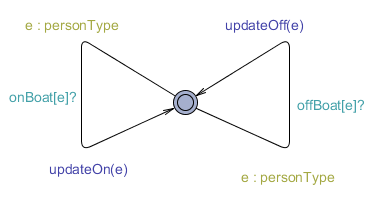
\includegraphics[width=\columnwidth]{pictures/observer.png}%
\caption{}%
\label{fig:observer}%
\end{figure}


